\chapter{Control system manual}

\section{System requirements}

The following is a list of all software required to run the control system implemented in this thesis. The are split into to parts, general software, python libraries and ROS-packages.

\begin{table}[H]
    \centering
    \begin{tabular*}{\linewidth}{ll}
    \toprule
    \multicolumn{2}{c}{\Large \textbf{\quad \quad \quad Requirements}} \\
    \midrule
    \multicolumn{2}{l}{\large \textbf{General}} \\
    \midrule
    Operating System & Ubuntu 20.04 LTS (Server version) \\
    ROS distrubution & Noetic \\ 
    Python &  3.8+ \\
    GCC & 8+ \\
    OpenCV & \\
    \midrule
    \multicolumn{2}{l}{\large \textbf{Python libraries}} \\
    \midrule
    Numpy 1.19.5+ & \\
    tensorflow & \\
    openCV & \\
    scipy & \\
    qp\_solvers & \\
    cvxopt & \\
    ds4drv & \\
    \midrule
    \multicolumn{2}{l}{\large \textbf{Ros packages}} \\
    \midrule
    CV-camera & \\
    CV-bridge & \\
    rplidar & \\
    rosserial & \\
    ds4\_drivers & \\
    dynamic\_reconfigure & \\
    \bottomrule
    \end{tabular*}
    \caption{Required software}
    \label{tab:requiredsoftware}
\end{table}

\section{Running the control system nodes}

This section will describe the procedure for running the available control system. First, one must SSH onto the raspberry pi as described in \cref{sec:commwithpi}. Den navigate to the workspace. It should be called \texttt{ws\_saucer}. Source the setup.bash file, and we are ready to start. 

\subsection{Dualshock 4 driver}
 
The system relies on the playstation ds4-driver, so we start by launching this node. Its package should be in the directory. To activate the driver, run the command

\begin{lstlisting}[language=bash]
$ roslaunch ds4_driver ds4_driver.launch use_standard_messages:=True
\end{lstlisting}

Running a roslaunch command will automatically start the ROS-master if you do not have one running. To connect the bluetooth controller, simply press the button on the middle. The controller should light blue when connected and an ouput should be printed in the terminal window. If the controller is not paired, you can follow this \underline{\href{https://ubuntu.com/core/docs/bluez/reference/pairing/outbound-pairing}{tutorial}}.


\subsection{Camera}
\label{sec:camera-driver}
Next up is the camera node. Open a new terminal. For this driver you do not have to be in the workspace. 

\begin{lstlisting}[language=bash]
$ rosrun cv_camera cv_camera_node
\end{lstlisting}

You should see an ouput that the calibration file was loaded if successfully activated. 

\subsection{Lidar}
\label{sec:lidar-driver}
To activate the lidar, open a new terminal and navigate to the workspace folder again. Then run the command

\begin{lstlisting}[language=bash]
$ roslaunch rplidar rplidar.launch 
\end{lstlisting}

Again, if successful you should see an output in the terminal. If it tells you the firmware is deprecated, just ignore the warning. 

\subsection{Arduino}

Finally, before we activate the motion control system we must enable one final node. This is the node on the Arduino that subscribes to the pwm signals. To enable it, run 

\begin{lstlisting}[language=bash]
$ rosrun rosserial_python serial_node.py _port=:dev/ttyACM0
\end{lstlisting}

Here the final argument specifies which usb port the arduino is connected to on the raspberry pi. It may vary, so to check run 

\begin{lstlisting}[language=bash]
$ ls /dev
\end{lstlisting}

to see which devices are connected. 

\subsection{Motion Control System}

Finally, we can activate the motion control system. In the workspace folder run 

\begin{lstlisting}[language=bash]
$ roslaunch feedback_controller collision_avoidance.launch
\end{lstlisting}

This should activate necessary nodes. The system defaults to manual control with the joystick controller, but can switch to automatic by pressing the triangle button on the ds4 controller. The guidance is activated by pressing square. Note that this should not be done unless the vessel is in the basin, and the object detection node is active. 

If one wishes to for example test one node, each package can be launched individually using the guidelines from \cref{sec:run-nodes}.

\subsection{Object detection}

On your operator computer, navigate to the workspace folder of your choice. Remember to export the ROS master url to establish communication between the nodes. To run the SA system use the following command

\begin{lstlisting}[language=bash]
$ rosrun objdetection detection_node
\end{lstlisting}

This will open a window with video-feed from the saucer on your operator computer. 


\section{Dynamic Reconfigure}

To make tuning your controller and observer more effective, tools for dynamic tuning are provided in the form of the ROS-package gain\_server. This allows you to change the gains in real time, rather than having to hard-code the gains and then stopping and starting your system every time you want to change them. To activate the node, and GUI use the following steps

Run the node use the command:
\begin{lstlisting}[language=bash]
$ rosrun gain_server server.py
\end{lstlisting}
\textbf{NOTE!} If you use the dynamic tuning, you should always activate this node \textbf{first} or you may experience errors. This is because the subscriberss in guidance, observer and controller nodes will expect values to be there when they are not. When the node is activated, the initial gains should be printed to your terminal. If you use the collision\_avoidance.launch file the gain\_server node will be started as part of this, and you can disregard the first step. 
    
 In another terminal, activate the GUI: 
\begin{lstlisting}[language=bash]
$ rosrun rqt_gui rqt_gui -s reconfigure
\end{lstlisting}
    
This should open a program that looks like this: 
    
\begin{figure}[H]
    \centering
    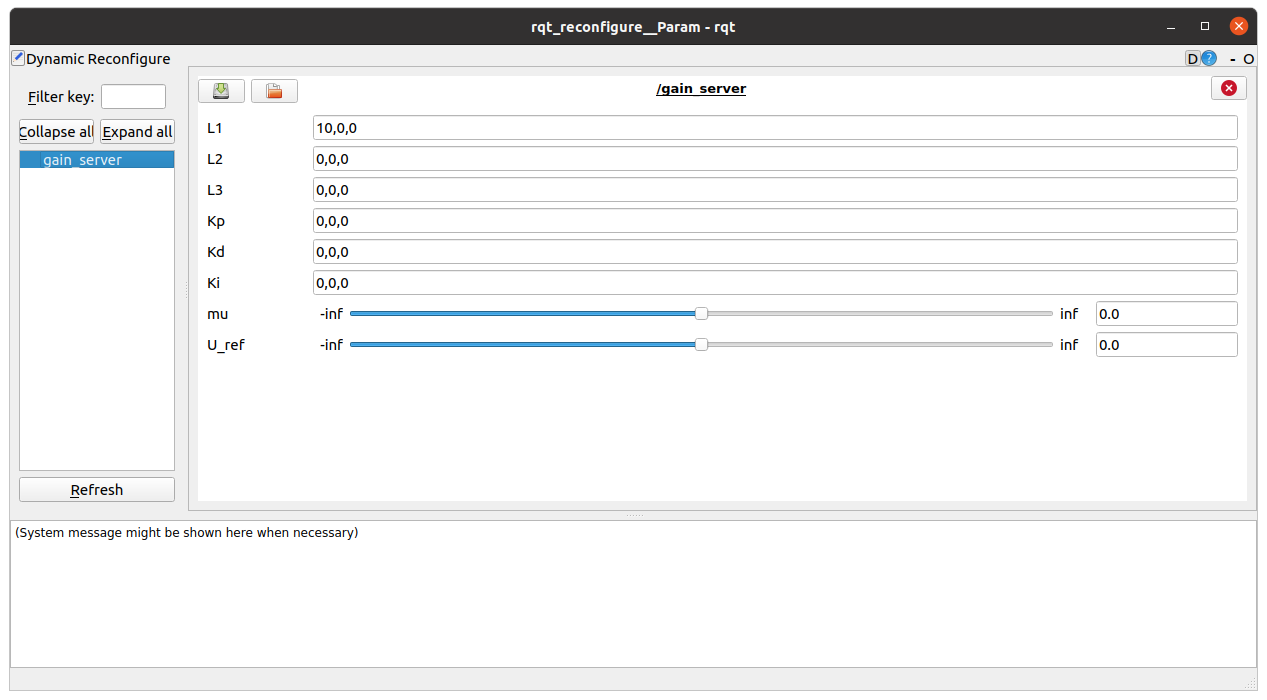
\includegraphics[width=\textwidth]{Images/dynamic-reconfigure.png}
    \caption{Tuning GUI}
    \label{fig:tuner}
\end{figure}
    
Each field or slider here corresponds to a gain in either the observer or controller. Not all the variables are relevant either. The last to are single float values, while the first six are meant to represent the elements on the diagonal of a $3\times3$-matrix. Change these to tune you controller. 
